\section{Model Adequacy Checking}


\begin{frame}{Assumptions Behind the Fitted Model}
    The linear model $\mathbf y=\mathbf X\boldsymbol\beta+\boldsymbol\varepsilon$ is fitted under five assumptions:
    \begin{itemize}
        \item The relationship between $y$ and the regressors is (approximately) linear
        \item $\mathrm{E}[\varepsilon_i]=0$
        \item $\mathrm{Var}(\varepsilon_i)=\sigma^2$ for all $i$ (constant variance)
        \item The errors are uncorrelated
        \item The errors are normally distributed (needed for the $t$ and $F$ procedures)
    \end{itemize}
    Least squares returns estimates whether or not these assumptions hold.
\end{frame}


\begin{frame}{What Can We Observe?}
    The errors $\varepsilon_i$ are never observed. What can we observe instead?

    % The residuals $e_i=y_i-\hat y_i$. If the model is adequate they behave approximately like the errors, so departures from the assumptions should show up in the residuals.
\end{frame}


\section{Raw Residuals}


\begin{frame}{Raw Residuals}
    The $i$th residual is $e_i=y_i-\hat y_i$. In matrix form
    \begin{align*}
        \mathbf e &= \mathbf y-\hat{\mathbf y} = (\mathbf I-\mathbf H)\mathbf y \\
        &= (\mathbf I-\mathbf H)\boldsymbol\varepsilon ,
    \end{align*}
    where the last step uses $(\mathbf I-\mathbf H)\mathbf X=\mathbf 0$.
\end{frame}


\begin{frame}{Leverage}
    The hat matrix is $\mathbf H=\mathbf X(\mathbf X^\top\mathbf X)^{-1}\mathbf X^\top$ with diagonal elements
    \[
        h_{ii}=\mathbf x_i^\top(\mathbf X^\top\mathbf X)^{-1}\mathbf x_i .
    \]
    \begin{itemize}
        \item Intuitively, $h_{ii}$ measures how far $\mathbf x_i$ is from the center of the regressor data: points with unusual $x$-values have more "leverage" to pull the fitted surface toward their own $y_i$
        \item $h_{ii}$ is large when $\mathbf x_i$ is far from the centroid of the regressor values
        \item $0\le h_{ii}\le 1$ and $\sum_{i=1}^n h_{ii}=p$, where $p$ is the number of model parameters
        \item $\hat y_i=\sum_j h_{ij}y_j$, so $h_{ii}$ is the weight of $y_i$ in its own fitted value
    \end{itemize}
\end{frame}


\begin{frame}{Flagging High-Leverage Points}
    Rule of thumb (MPV): observation $i$ has high leverage if
    \[
        h_{ii} > \frac{2p}{n} .
    \]
    \begin{itemize}
        \item Delivery time data: $p=3$, $n=25$, so the cutoff is $2p/n = 2(3)/25 = 0.24$
        \item Observation 9: $h_{99}=0.498 > 0.24$, flagged as high leverage
        \item High leverage is about an unusual $\mathbf x_i$, not an unusual $y_i$: a flagged point can still have a small residual if $y_i$ happens to agree with the trend at that $\mathbf x_i$
    \end{itemize}
\end{frame}


\begin{frame}{Leverage: Geometric Intuition}
    \begin{columns}[T]
        \column{0.45\textwidth}
        \begin{itemize}
            \item Leverage depends only on the location of $\mathbf x_i$, not on $y_i$
            \item A point far from $\bar x$ has high leverage, whatever its $y$-value
            \item Here the flagged point sits far from the rest of the data in $x$, yet close to the fitted line: high leverage, small residual
        \end{itemize}
        \column{0.52\textwidth}
        \centering
        \mode<presentation>{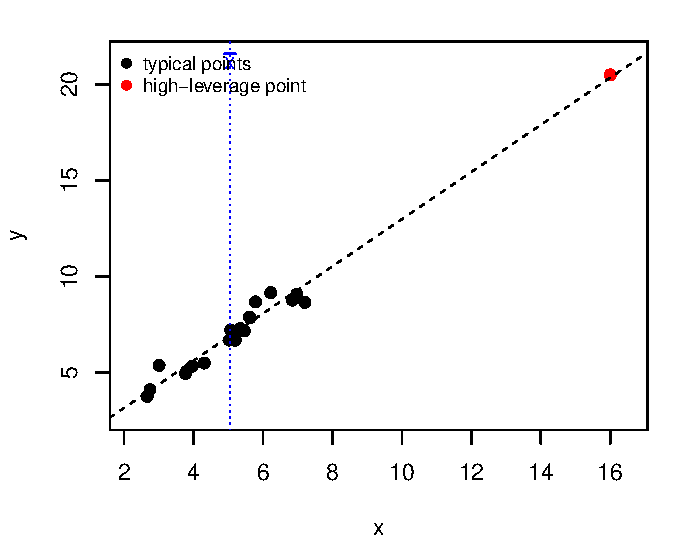
\includegraphics[width=\linewidth]{figures/leverage-geometry}}\mode<article>{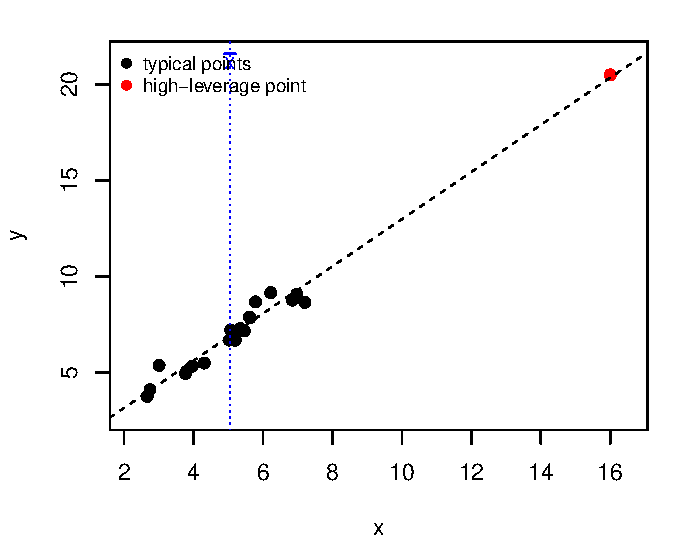
\includegraphics[width=0.7\linewidth]{figures/leverage-geometry}}
    \end{columns}
\end{frame}


\begin{frame}{Mean and Covariance of the Residuals}
    \begin{align}
        \mathrm{E}[\mathbf e] &= \mathbf 0 \notag \\
        \mathrm{Var}(\mathbf e) &= \sigma^2(\mathbf I-\mathbf H) \label{eq:var-e}
    \end{align}
    Element by element
    \begin{align*}
        \mathrm{Var}(e_i) &= \sigma^2(1-h_{ii}) \\
        \mathrm{Cov}(e_i,e_j) &= -\sigma^2 h_{ij}, \qquad i\neq j .
    \end{align*}
\end{frame}


\begin{frame}{Are the Residuals iid?}
    The errors are assumed iid $N(0,\sigma^2)$. Are the residuals $e_1,\dots,e_n$ iid?

    % No. $\mathrm{Var}(e_i)=\sigma^2(1-h_{ii})$ differs across $i$ whenever the $h_{ii}$ differ, $\mathrm{Cov}(e_i,e_j)=-\sigma^2h_{ij}\neq 0$, and the residuals satisfy the $p$ linear constraints $\mathbf X^\top\mathbf e=\mathbf 0$ (in particular $\sum_i e_i=0$ when the model has an intercept).
\end{frame}


\section{Standardized Residuals}


\begin{frame}{Standardized Residuals}
    \begin{align}
        d_i = \frac{e_i}{\sqrt{\text{MSE}}}, \qquad \text{MSE}=\frac{\text{SS}_{\text{Res}}}{n-p} \label{eq:d}
    \end{align}
    \begin{itemize}
        \item $\mathrm{E}[d_i]=0$ and $\mathrm{Var}(d_i)\approx 1$, and $d_i$ is free of the units of $y$
        \item Rule of thumb: $|d_i|>3$ marks a potential outlier
        \item $d_i$ ignores that $\mathrm{Var}(e_i)=\sigma^2(1-h_{ii})$ differs across observations, see \eqref{eq:var-e}
    \end{itemize}
\end{frame}


\section{Studentized Residuals}


\begin{frame}{Studentized Residuals}
    \begin{align}
        r_i = \frac{e_i}{\sqrt{\text{MSE}\,(1-h_{ii})}} = \frac{d_i}{\sqrt{1-h_{ii}}} \label{eq:r}
    \end{align}
    \begin{itemize}
        \item Divides $e_i$ by its own estimated standard deviation from \eqref{eq:var-e}, so $\mathrm{Var}(r_i)=1$ for every $i$, whatever the location of $\mathbf x_i$
        \item $|r_i|\ge|d_i|$, with $d_i$ from \eqref{eq:d}
        \item $r_i\approx d_i$ when $h_{ii}$ is small, and they differ noticeably for high-leverage points
    \end{itemize}
\end{frame}


\begin{frame}{Leverage and Residual Size}
    Points with large leverage tend to have small raw residuals. Why?

    % A large $h_{ii}$ pulls the fitted surface toward $y_i$, since $\hat y_i=\sum_j h_{ij}y_j$ contains $h_{ii}y_i$. Formally $\mathrm{Var}(e_i)=\sigma^2(1-h_{ii})\to 0$ as $h_{ii}\to 1$, so $e_i$ understates how far $y_i$ is from where the rest of the data would put it.
\end{frame}


\section{PRESS Residuals}


\begin{frame}{Leave-One-Out Prediction Error}
    The PRESS residual is the error when $y_i$ is predicted from the model fitted to the other $n-1$ observations
    \[
        e_{(i)} = y_i-\hat y_{(i)} = \frac{e_i}{1-h_{ii}} .
    \]
    \begin{itemize}
        \item The identity avoids refitting the model $n$ times
        \item A large $h_{ii}$ inflates the gap between $e_{(i)}$ and $e_i$
    \end{itemize}
\end{frame}


\begin{frame}{Variance of PRESS Residuals and the PRESS Statistic}
    \begin{align*}
        \mathrm{Var}(e_{(i)}) &= \frac{\sigma^2}{1-h_{ii}} \\
        \text{PRESS} &= \sum_{i=1}^n e_{(i)}^2
    \end{align*}
    \begin{itemize}
        \item PRESS measures predictive ability: smaller is better
        \item Standardizing $e_{(i)}$ by its standard deviation returns the studentized residual
    \end{itemize}
    \[
        \frac{e_{(i)}}{\sqrt{\mathrm{Var}(e_{(i)})}} = \frac{e_i}{\sqrt{\sigma^2(1-h_{ii})}}
    \]
\end{frame}


\section{R-Student Residuals}


\begin{frame}{Removing Observation $i$ From the Variance Estimate}
    MSE uses all $n$ observations, including observation $i$: a large $e_i$ inflates MSE and shrinks $r_i$. Instead use the variance estimate from the fit without observation $i$
    \begin{align}
        S_{(i)}^2 = \frac{(n-p)\,\text{MSE} - e_i^2/(1-h_{ii})}{n-p-1} , \label{eq:s2i}
    \end{align}
    which also needs no refit.
\end{frame}


\begin{frame}{R-Student Residuals}
    \[
        t_i = \frac{e_i}{\sqrt{S_{(i)}^2\,(1-h_{ii})}}
    \]
    \begin{itemize}
        \item Replaces MSE in \eqref{eq:r} by $S_{(i)}^2$ from \eqref{eq:s2i}
        \item If the errors are normal, $t_i\sim t_{n-p-1}$
        \item More sensitive to an outlier than $r_i$: the outlier no longer inflates its own denominator
        \item Used to test for outliers (later lecture)
    \end{itemize}
\end{frame}


\begin{frame}{Types of Residuals}
    \mode<presentation>{\footnotesize}
    \begin{center}
        \begin{tabular}{llll}
            \toprule
            Residual & Formula & Variance / distribution & Note \\
            \midrule
            Raw & $e_i$ & $\sigma^2(1-h_{ii})$ & Unequal variances \\
            Standardized & $e_i/\sqrt{\text{MSE}}$ & $\approx 1$ & Ignores $h_{ii}$ \\
            Studentized & $e_i/\sqrt{\text{MSE}(1-h_{ii})}$ & $1$ & Accounts for leverage \\
            PRESS & $e_i/(1-h_{ii})$ & $\sigma^2/(1-h_{ii})$ & Leave-one-out error \\
            R-student & $e_i/\sqrt{S_{(i)}^2(1-h_{ii})}$ & $t_{n-p-1}$ & Outlier detection \\
            \bottomrule
        \end{tabular}
    \end{center}
\end{frame}


\section{Example: Delivery Time Data}


\begin{frame}{Delivery Time Data}
    \begin{itemize}
        \item $y$: delivery time (minutes) of a route driver servicing vending machines
        \item $x_1$: number of cases of product stocked
        \item $x_2$: distance walked by the driver (feet)
        \item $n=25$ observations, $p=3$
    \end{itemize}
    Fitted model
    \[
        \hat y = 2.341 + 1.616\,x_1 + 0.0144\,x_2, \qquad \text{MSE}=10.624, \quad \hat\sigma=3.259 .
    \]
\end{frame}


\begin{frame}{Delivery Time Data: Residuals}
    \small
    \begin{center}
        \begin{tabular}{rrrrrrr}
            \toprule
            $i$ & $h_{ii}$ & $e_i$ & $d_i$ & $r_i$ & $e_{(i)}$ & $t_i$ \\
            \midrule
            1 & 0.102 & $-5.028$ & $-1.543$ & $-1.628$ & $-5.598$ & $-1.696$ \\
            9 & 0.498 & $7.420$ & $2.276$ & $3.214$ & $14.789$ & $4.311$ \\
            10 & 0.196 & $2.376$ & $0.729$ & $0.813$ & $2.957$ & $0.807$ \\
            15 & 0.041 & $0.671$ & $0.206$ & $0.210$ & $0.700$ & $0.206$ \\
            20 & 0.102 & $-5.788$ & $-1.776$ & $-1.874$ & $-6.443$ & $-1.997$ \\
            22 & 0.392 & $-3.687$ & $-1.131$ & $-1.450$ & $-6.059$ & $-1.490$ \\
            \bottomrule
        \end{tabular}
    \end{center}
    Six of the 25 observations. $d_i$ standardized, $r_i$ studentized, $e_{(i)}$ PRESS, $t_i$ R-student. $\text{PRESS}=459.04$.
\end{frame}


\begin{frame}{Observation 9}
    Observation 9 (30 cases, 1460 ft) has the largest leverage, $h_{99}=0.498$. Its residuals are $d_9=2.276$, $r_9=3.214$, $t_9=4.311$. Why does the residual keep growing from $d_9$ to $r_9$ to $t_9$?

    % $r_9=d_9/\sqrt{1-h_{99}}=d_9/0.708$: high leverage shrinks $\mathrm{Var}(e_9)$, so the raw residual understates how unusual the point is. $t_9$ replaces $\text{MSE}=10.624$ by $S_{(9)}^2=5.905$, the variance estimate without observation 9 itself: the outlier no longer inflates the denominator.
\end{frame}


\section{Normality}


\subsection{Normal Probability Plot}


\begin{frame}{Normal Probability Plot: Construction}
    \begin{itemize}
        \item Order the residuals: $e_{[1]}\le e_{[2]}\le\dots\le e_{[n]}$
        \item Plot $e_{[i]}$ against the normal quantile $\Phi^{-1}\!\left(\dfrac{i-1/2}{n}\right)$
        \item If the errors are normal, the points fall close to a straight line
        \item Use studentized or R-student residuals so that all residuals have the same variance
    \end{itemize}
\end{frame}


\begin{frame}{Normal Probability Plot: Patterns}
    \begin{columns}[T]
        \column{0.42\textwidth}
        \begin{itemize}
            \item Straight line: consistent with normality
            \item Heavy tails: ends bend away from the line (S-shape)
            \item Light tails: ends bend toward the center (reversed S)
            \item Skewness: one-sided curvature
            \item Isolated points at the ends: outliers
        \end{itemize}
        \column{0.55\textwidth}
        \centering
        \mode<presentation>{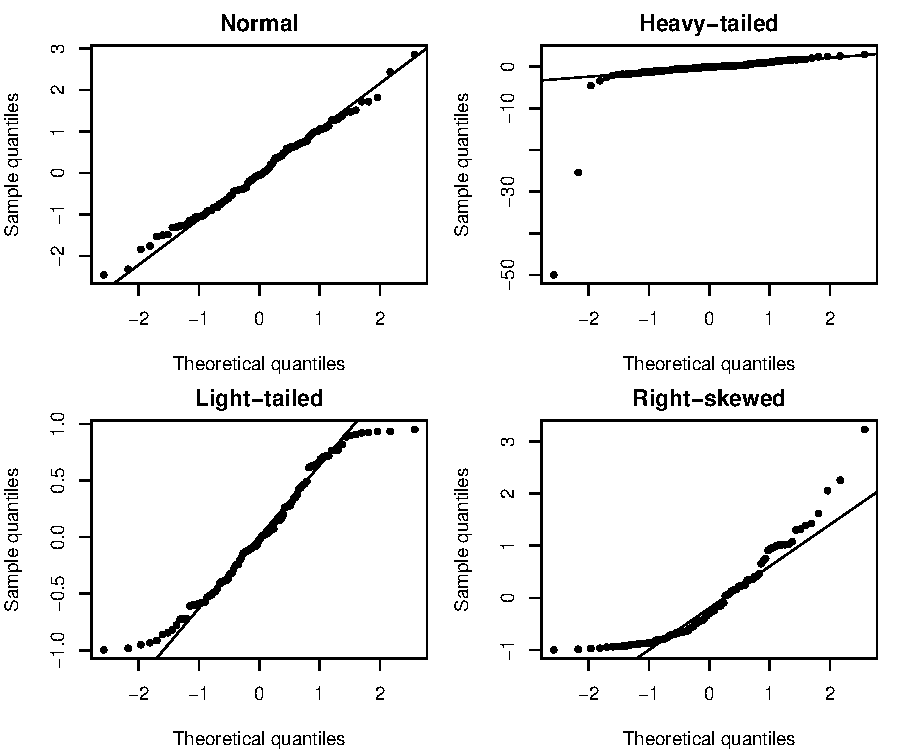
\includegraphics[width=\linewidth]{figures/qq-patterns}}\mode<article>{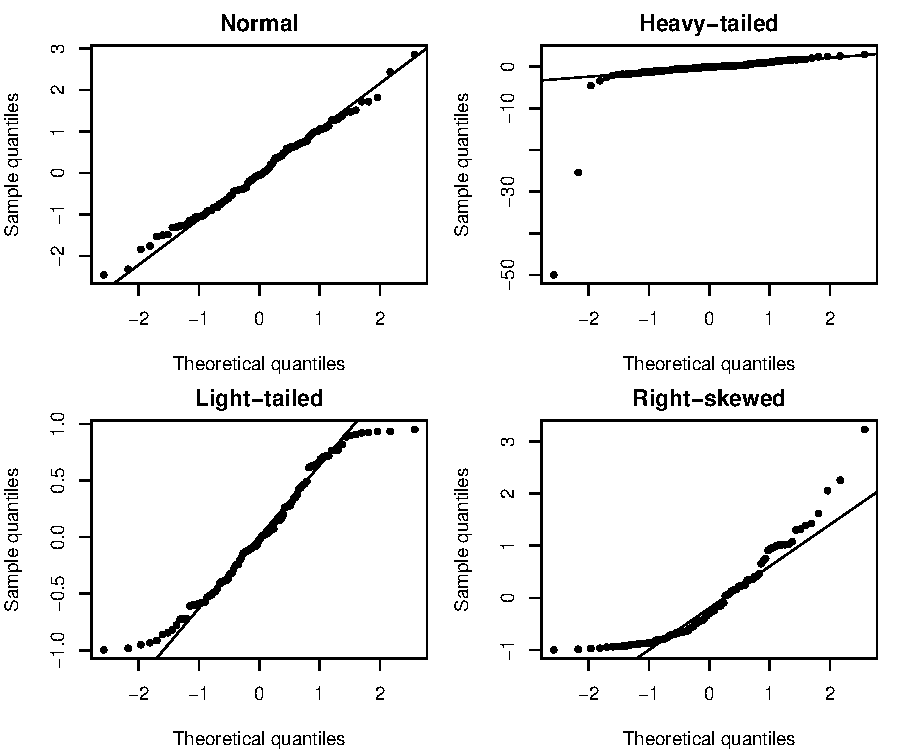
\includegraphics[width=0.8\linewidth]{figures/qq-patterns}}
    \end{columns}
\end{frame}


\begin{frame}{Normal Probability Plot: Delivery Time Data}
    \begin{columns}[T]
        \column{0.45\textwidth}
        \begin{itemize}
            \item The central points follow the line
            \item Observation 9 ($r_9=3.21$) lies far above the line in the upper tail
            \item Is the departure from normality serious, or is it one point?
        \end{itemize}
        \column{0.52\textwidth}
        \centering
        \mode<presentation>{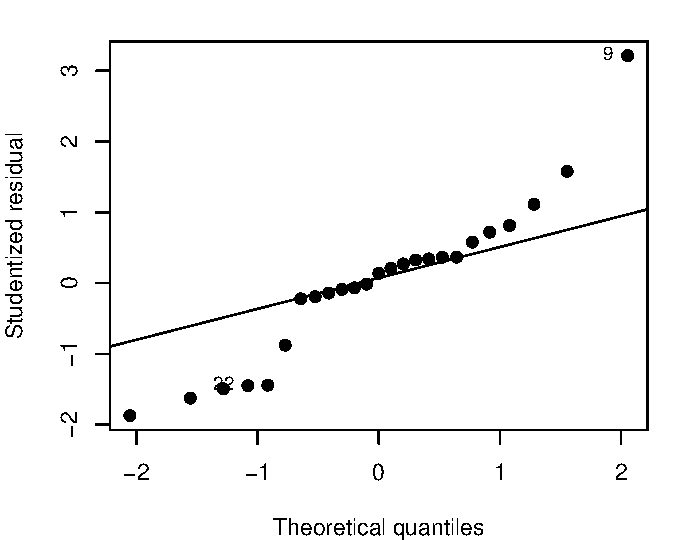
\includegraphics[width=\linewidth]{figures/qq-delivery}}\mode<article>{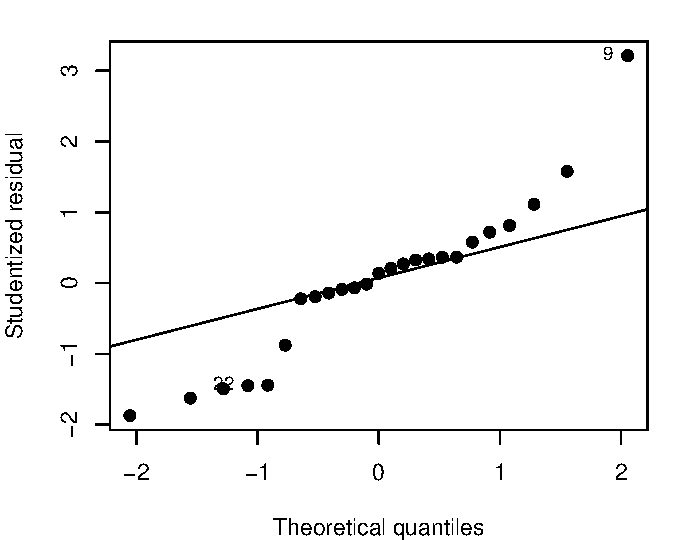
\includegraphics[width=0.7\linewidth]{figures/qq-delivery}}
    \end{columns}
\end{frame}


\subsection{Shapiro--Wilk Test}


\begin{frame}{Shapiro--Wilk Test}
    $H_0$: the errors are normally distributed, against $H_1$: they are not.
    \[
        W=\frac{\left(\sum_{i=1}^n a_i\,e_{[i]}\right)^2}{\sum_{i=1}^n (e_i-\bar e)^2}
    \]
    \begin{itemize}
        \item $e_{[i]}$ are the ordered residuals; the constants $a_i$ come from the expected order statistics of a normal sample and are supplied by software
        \item $W$ is closely related to the squared correlation between ordered residuals and normal scores
        \item $0<W\le 1$: values near 1 are consistent with normality, small $W$ rejects $H_0$
    \end{itemize}
\end{frame}


\begin{frame}{Test or Plot?}
    With $n=100{,}000$ the Shapiro--Wilk test rejects for negligible departures from normality; with $n=10$ it rarely rejects. Which should we trust, the test or the plot?

    % Neither alone. The plot shows the kind and size of the departure; the test only measures how strong the evidence is, which depends heavily on $n$. Look at the plot first, then use the test to back up what the plot suggests.
\end{frame}


\begin{frame}{Delivery Time Data: Shapiro--Wilk}
    Applied to the studentized residuals: $W=0.923$, $p=0.060$.
    \begin{itemize}
        \item Do not reject normality at the 5\% level, but the evidence is borderline
        \item The plot located the problem: observation 9
        \item Refitting without observation 9 (diagnostic only): $W=0.970$, $p=0.68$
    \end{itemize}
\end{frame}


\section{Constant Variance}


\subsection{Residuals Against Fitted Values}


\begin{frame}{Residuals Against Fitted Values}
    \begin{itemize}
        \item Plot $r_i$ (or $e_i$) against $\hat y_i$
        \item If the model is adequate, the points form a horizontal band around zero with no structure
        \item Any systematic pattern points to a violated assumption
    \end{itemize}
    Why $\hat y_i$ and not $y_i$?

    % $\mathrm{Cov}(\mathbf e,\hat{\mathbf y})=\mathbf 0$, but $\mathrm{Cov}(\mathbf e,\mathbf y)=\sigma^2(\mathbf I-\mathbf H)\neq\mathbf 0$. Plotting against $y_i$ builds in a spurious positive relation between residual and abscissa.
\end{frame}


\begin{frame}{Pattern (a): Satisfactory}
    \begin{columns}[T]
        \column{0.45\textwidth}
        \begin{itemize}
            \item Horizontal band centered at zero
            \item No trend, no change in spread
            \item No evidence against linearity or constant variance
        \end{itemize}
        \column{0.52\textwidth}
        \centering
        \mode<presentation>{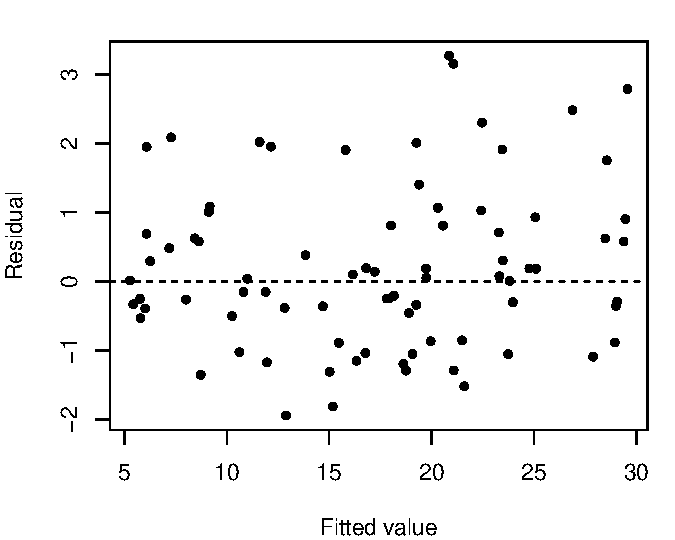
\includegraphics[width=\linewidth]{figures/pat-ok}}\mode<article>{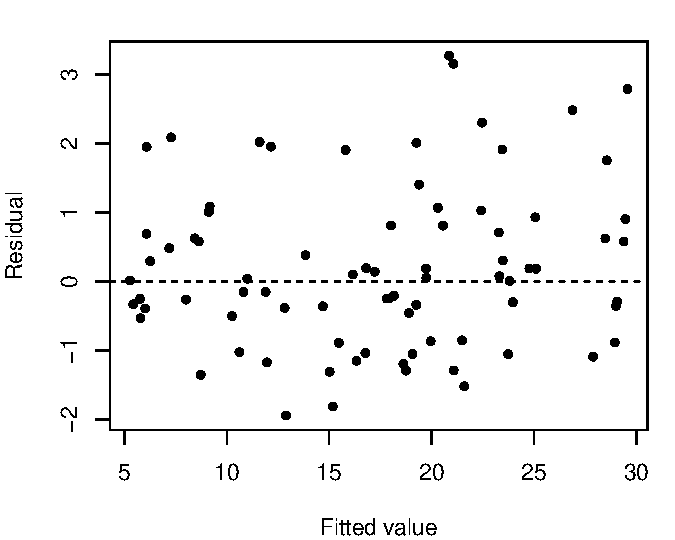
\includegraphics[width=0.7\linewidth]{figures/pat-ok}}
    \end{columns}
\end{frame}


\begin{frame}{Pattern (b): Funnel}
    \begin{columns}[T]
        \column{0.45\textwidth}
        \begin{itemize}
            \item Spread of the residuals grows with $\hat y_i$
            \item The variance is not constant, typically $\mathrm{Var}(y)$ increases with $\mathrm{E}(y)$
            \item Remedies: variance-stabilizing transformation of $y$, weighted least squares
        \end{itemize}
        \column{0.52\textwidth}
        \centering
        \mode<presentation>{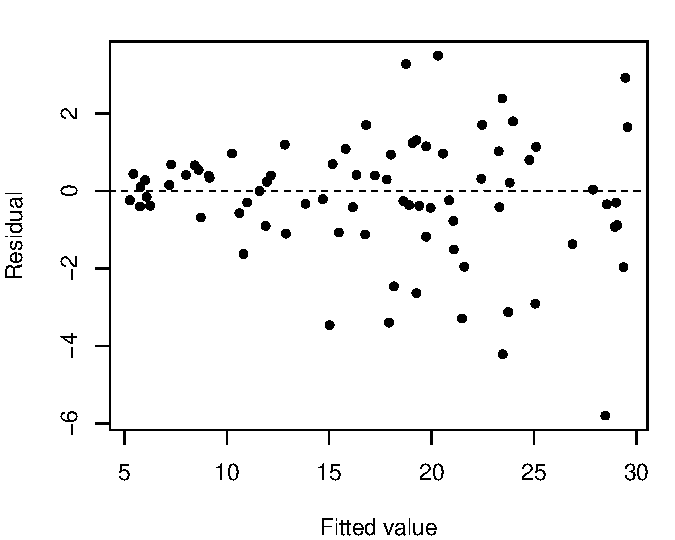
\includegraphics[width=\linewidth]{figures/pat-funnel}}\mode<article>{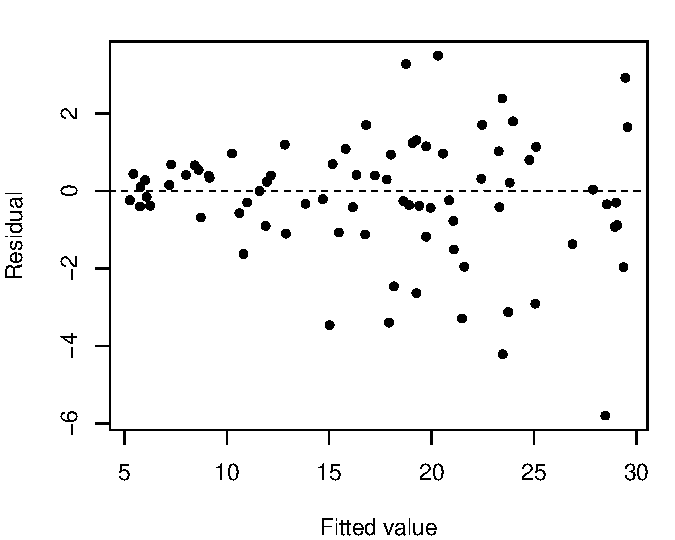
\includegraphics[width=0.7\linewidth]{figures/pat-funnel}}
    \end{columns}
\end{frame}


\begin{frame}{Pattern (c): Double Bow}
    \begin{columns}[T]
        \column{0.45\textwidth}
        \begin{itemize}
            \item Spread is largest in the middle and smallest at both ends
            \item Typical when $y$ is a proportion in $(0,1)$, where $\mathrm{Var}(y)\propto p(1-p)$
            \item Remedy: transformation of $y$
        \end{itemize}
        \column{0.52\textwidth}
        \centering
        \mode<presentation>{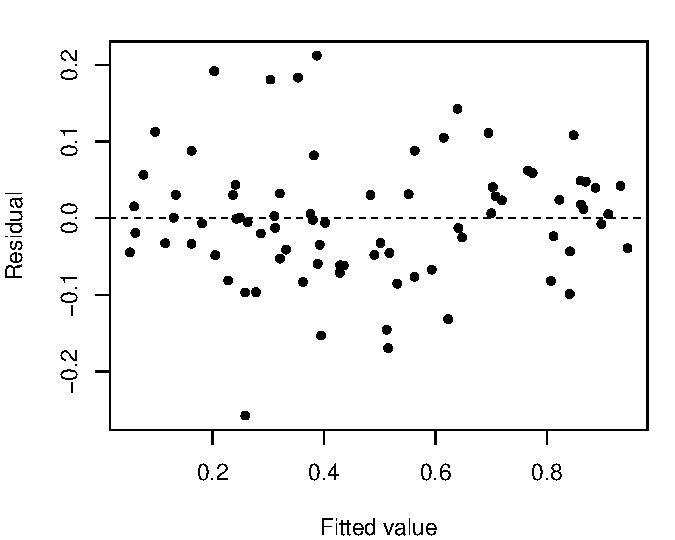
\includegraphics[width=\linewidth]{figures/pat-bow}}\mode<article>{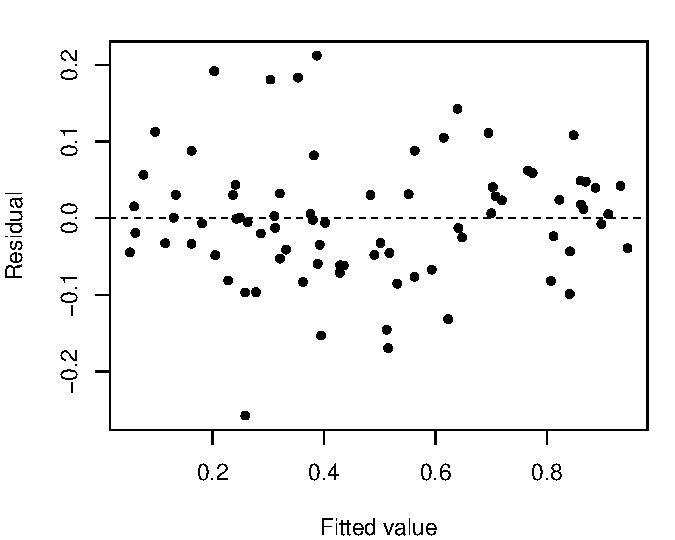
\includegraphics[width=0.7\linewidth]{figures/pat-bow}}
    \end{columns}
\end{frame}


\begin{frame}{Delivery Time Data: Residuals Against $\hat y_i$}
    \begin{columns}[T]
        \column{0.45\textwidth}
        \begin{itemize}
            \item Most points form a roughly horizontal band
            \item Observations 9 and 22 stand apart at large fitted values
            \item Is the spread at large $\hat y_i$ real, or driven by these two points?
        \end{itemize}
        \column{0.52\textwidth}
        \centering
        \mode<presentation>{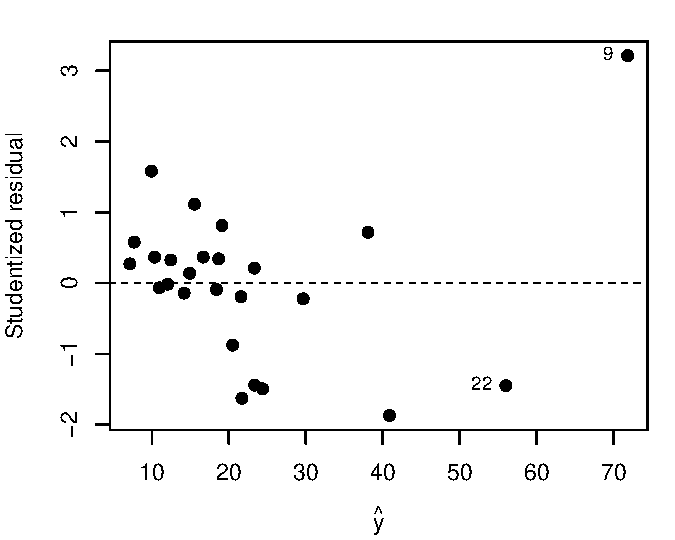
\includegraphics[width=\linewidth]{figures/rvf-delivery}}\mode<article>{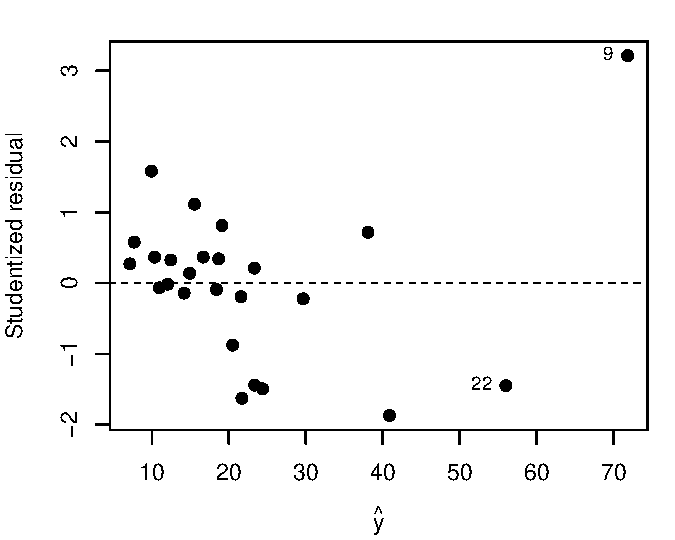
\includegraphics[width=0.7\linewidth]{figures/rvf-delivery}}
    \end{columns}
\end{frame}


\begin{frame}{Name the Violation}
    Which assumption does each plot call into question?
    \begin{columns}[T]
        \column{0.5\textwidth}
        \centering
        (a)\par
        \mode<presentation>{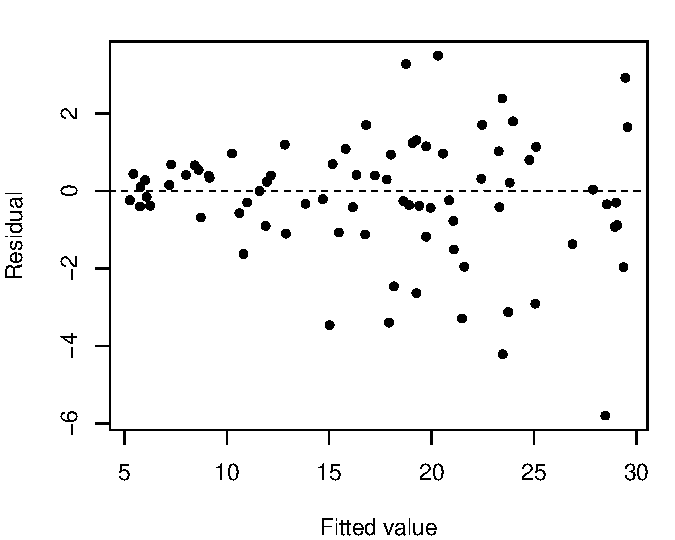
\includegraphics[height=0.6\textheight]{figures/pat-funnel}}\mode<article>{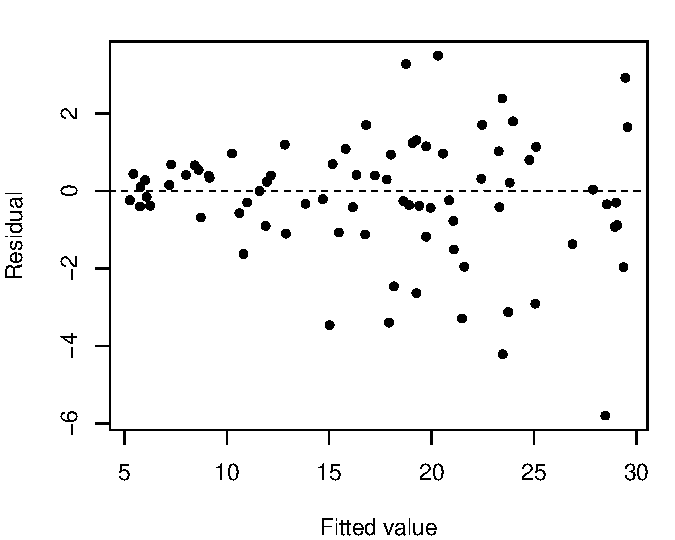
\includegraphics[width=0.6\linewidth]{figures/pat-funnel}}
        \column{0.5\textwidth}
        \centering
        (c)\par
        \mode<presentation>{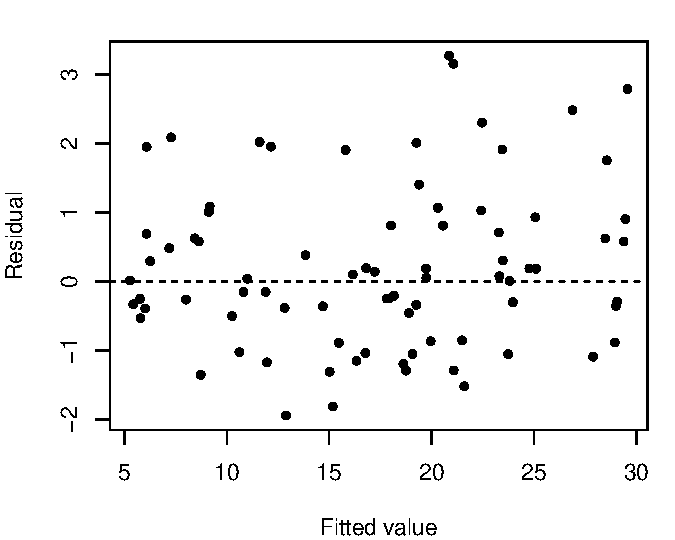
\includegraphics[height=0.6\textheight]{figures/pat-ok}}\mode<article>{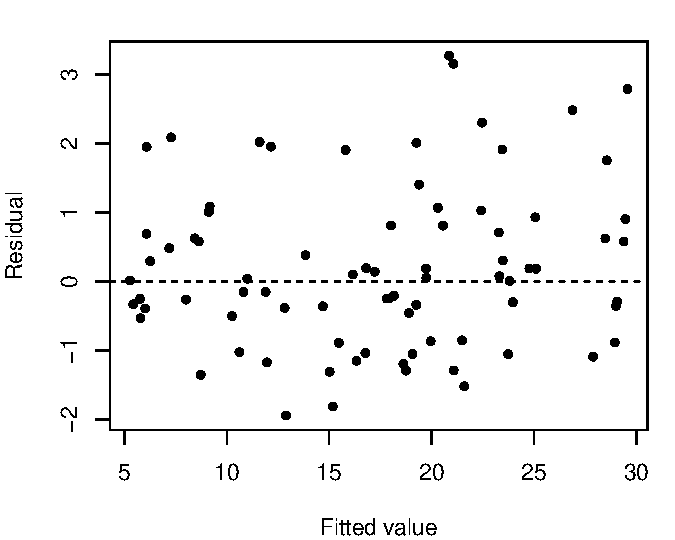
\includegraphics[width=0.6\linewidth]{figures/pat-ok}}
    \end{columns}

    % (a) funnel: nonconstant variance increasing with the mean. (c) satisfactory: no evidence against constant variance.
\end{frame}


\subsection{Breusch--Pagan and White Tests}


\begin{frame}{Why a Test?}
    A funnel plot is a judgment call. Formal tests of
    \begin{align*}
        H_0&: \mathrm{Var}(\varepsilon_i)=\sigma^2 \text{ for all } i \\
        H_1&: \text{the variance depends on the regressors}
    \end{align*}
    Two common choices: Breusch--Pagan and White.
\end{frame}


\begin{frame}{Breusch--Pagan Test}
    \begin{enumerate}
        \item Fit the model and obtain the residuals $e_i$
        \item Regress $e_i^2$ on the $k$ regressors and record $R^2_{\text{aux}}$
        \item Compute $LM=n\,R^2_{\text{aux}}$
        \item Under $H_0$, $LM\sim\chi^2_k$ approximately for large $n$; reject for large $LM$
    \end{enumerate}
    This is the studentized form, the default in \texttt{bptest} in R.
\end{frame}


\begin{frame}{White Test}
    Same steps as Breusch--Pagan, but the auxiliary regression of $e_i^2$ uses the regressors, their squares and their cross-products. For $k=2$ regressors
    \[
        e_i^2 \text{ on } x_1,\ x_2,\ x_1^2,\ x_2^2,\ x_1x_2 \quad\Longrightarrow\quad LM\sim\chi^2_5 .
    \]
    \begin{itemize}
        \item No assumption on the form of the heteroscedasticity
        \item Many auxiliary regressors when $k$ is large, which lowers power
    \end{itemize}
\end{frame}


\begin{frame}{Delivery Time Data: Tests for Nonconstant Variance}
    \begin{center}
        \begin{tabular}{lrrr}
            \toprule
            Test & $LM$ & df & $p$-value \\
            \midrule
            Breusch--Pagan & 11.99 & 2 & 0.0025 \\
            White & 14.96 & 5 & 0.0105 \\
            \bottomrule
        \end{tabular}
    \end{center}
    \begin{itemize}
        \item Both reject constant variance at the 5\% level
        \item The rejection is driven by observation 9: refitting without it (diagnostic only) gives Breusch--Pagan $LM=3.22$, $p=0.20$
    \end{itemize}
\end{frame}


\begin{frame}{If the Variance Is Not Constant}
    \begin{itemize}
        \item Variance-stabilizing transformation of $y$
        \item Weighted least squares (WLS)
    \end{itemize}
    Before either, check whether a single unusual observation, as in the delivery time data, produced the rejection.
\end{frame}


\section{Linearity of the Mean Function}


\subsection{Residuals Against Fitted Values}


\begin{frame}{Pattern (d): Curvature}
    \begin{columns}[T]
        \column{0.45\textwidth}
        \begin{itemize}
            \item Residuals are systematically positive in one range of $\hat y_i$ and negative in another
            \item The mean function is wrong: the linear model is inadequate
            \item Remedies: add higher-order or interaction terms, transform the regressors or $y$
        \end{itemize}
        \column{0.52\textwidth}
        \centering
        \mode<presentation>{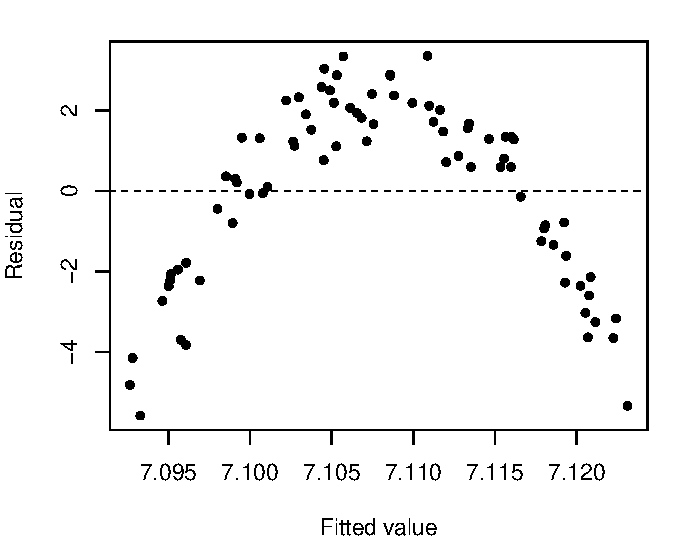
\includegraphics[width=\linewidth]{figures/pat-nonlinear}}\mode<article>{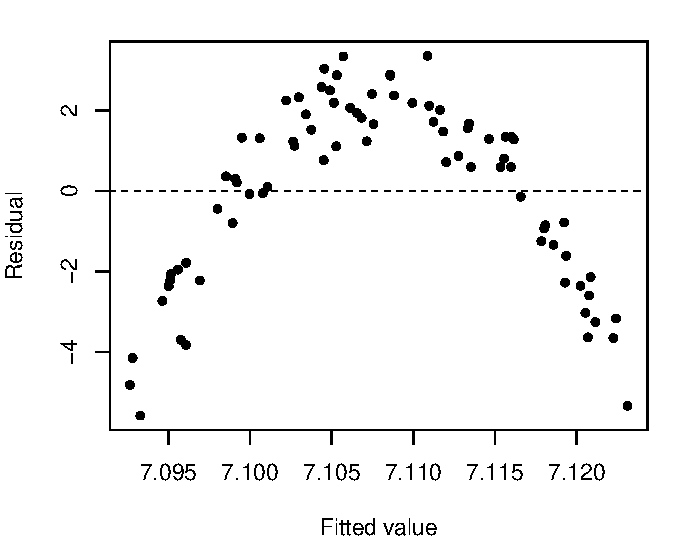
\includegraphics[width=0.7\linewidth]{figures/pat-nonlinear}}
    \end{columns}
\end{frame}


\begin{frame}{Name the Violation}
    Which assumption does each plot call into question?
    \begin{columns}[T]
        \column{0.5\textwidth}
        \centering
        (i)\par
        \mode<presentation>{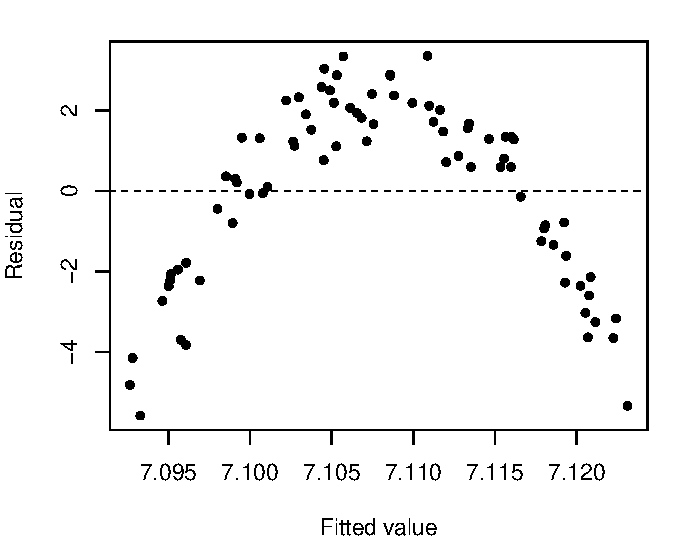
\includegraphics[height=0.6\textheight]{figures/pat-nonlinear}}\mode<article>{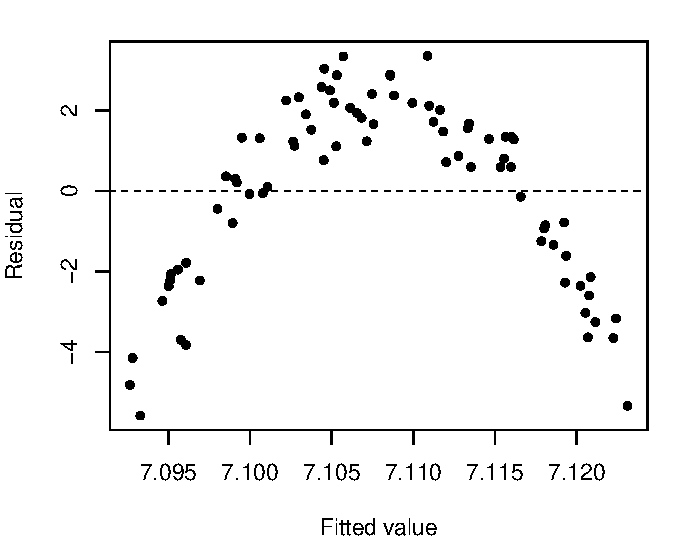
\includegraphics[width=0.6\linewidth]{figures/pat-nonlinear}}
        \column{0.5\textwidth}
        \centering
        (ii)\par
        \mode<presentation>{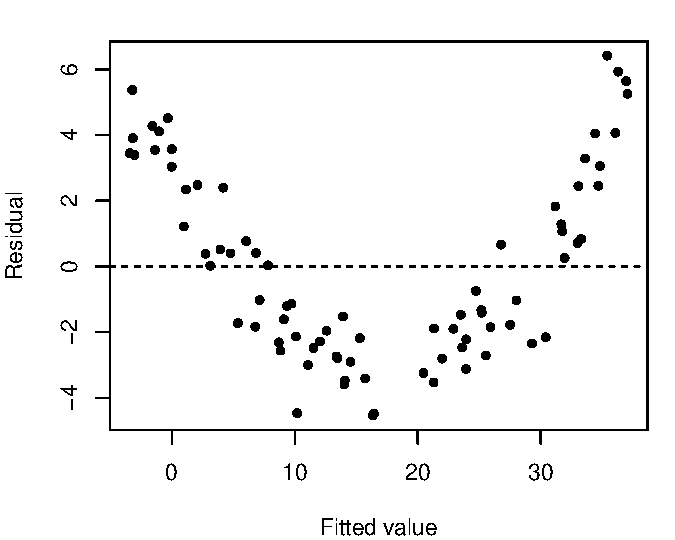
\includegraphics[height=0.6\textheight]{figures/pat-nonlinear2}}\mode<article>{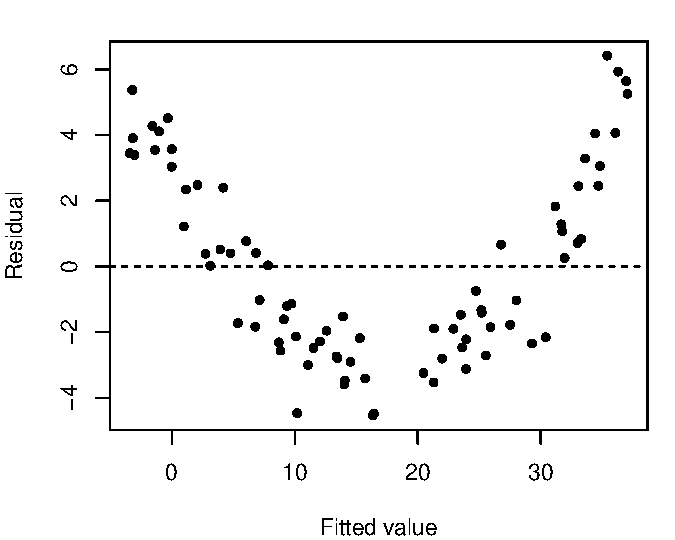
\includegraphics[width=0.6\linewidth]{figures/pat-nonlinear2}}
    \end{columns}

    % Both show curvature: the mean function is wrong in both cases, just bowing in opposite directions. (i) suggests a negative quadratic term is missing; (ii) suggests a positive one. Either way the linear model is inadequate.
\end{frame}


\subsection{Residuals Against Regressors}


\begin{frame}{Residuals Against Regressors}
    Plot $r_i$ against each regressor $x_j$.
    \begin{itemize}
        \item Curvature: $x_j$ enters the mean function in a nonlinear way, add a higher-order term or transform $x_j$
        \item Funnel: the variance depends on $x_j$
        \item A plot against a regressor not in the model: a pattern means that regressor should be added
    \end{itemize}
\end{frame}


\begin{frame}{Delivery Time Data: Residuals Against $x_1$ and $x_2$}
    \begin{columns}[T]
        \column{0.5\textwidth}
        \centering
        \mode<presentation>{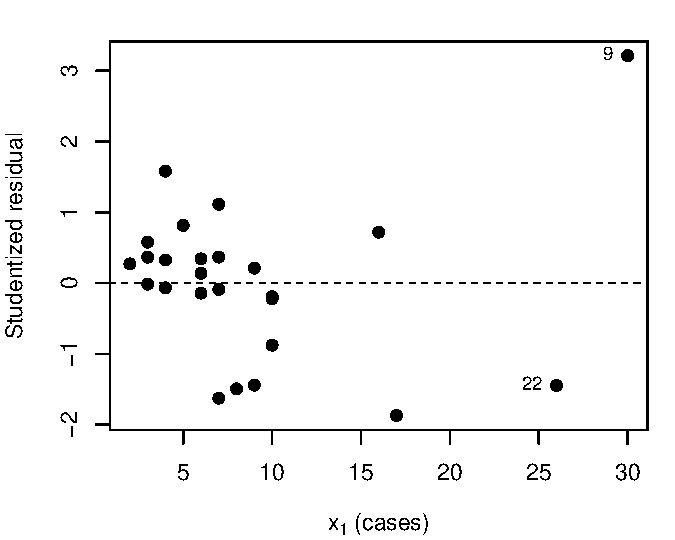
\includegraphics[width=\linewidth]{figures/rvx1-delivery}}\mode<article>{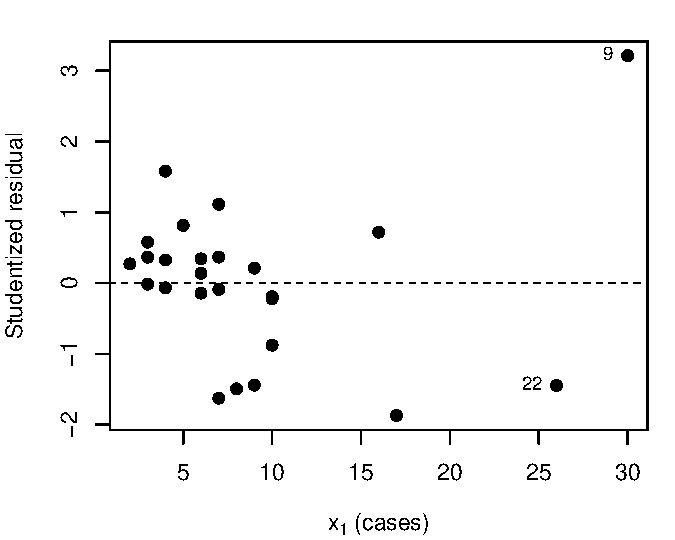
\includegraphics[width=0.8\linewidth]{figures/rvx1-delivery}}
        \column{0.5\textwidth}
        \centering
        \mode<presentation>{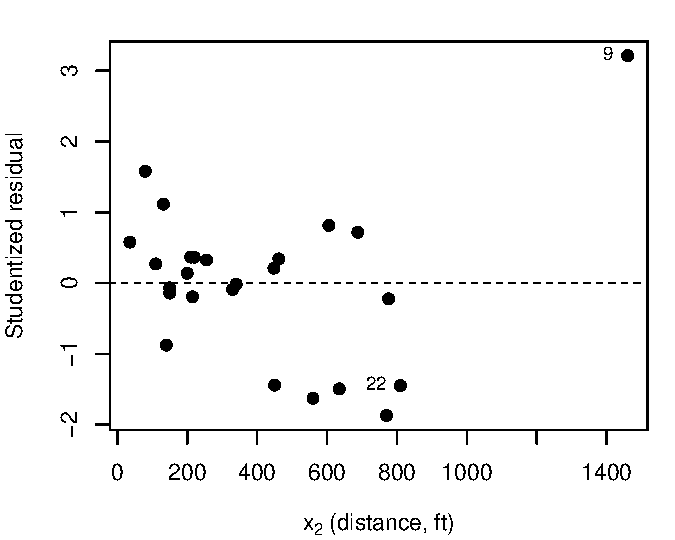
\includegraphics[width=\linewidth]{figures/rvx2-delivery}}\mode<article>{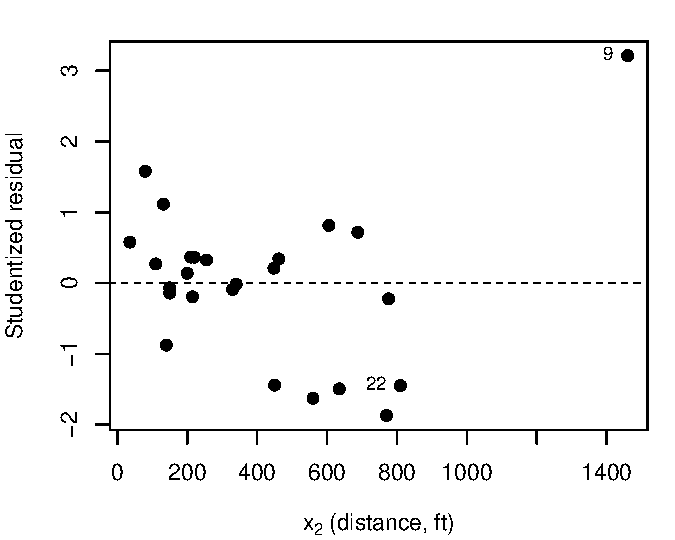
\includegraphics[width=0.8\linewidth]{figures/rvx2-delivery}}
    \end{columns}
    Neither plot shows clear curvature. Observation 9 is isolated at the extreme of both regressors.
\end{frame}


\section{Uncorrelated Errors}


\subsection{Residuals Against Time Order}


\begin{frame}{Residuals Against Time Order}
    Plot $e_t$ (or $r_t$) against the order in which the data were collected.
    \begin{columns}[T]
        \column{0.5\textwidth}
        \centering
        \mode<presentation>{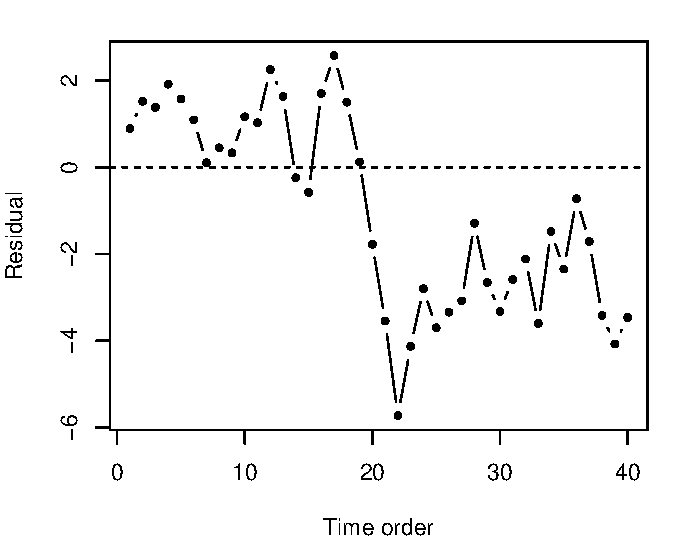
\includegraphics[width=0.75\linewidth]{figures/time-positive}}\mode<article>{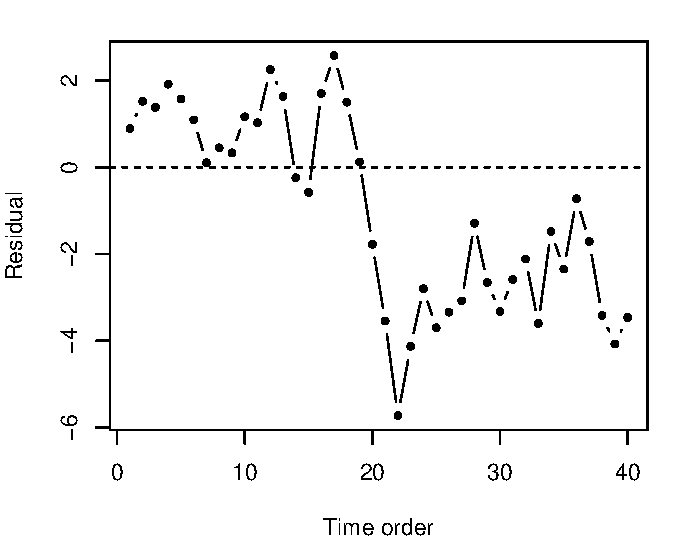
\includegraphics[width=0.8\linewidth]{figures/time-positive}}

        Positive autocorrelation: long runs of one sign.
        \column{0.5\textwidth}
        \centering
        \mode<presentation>{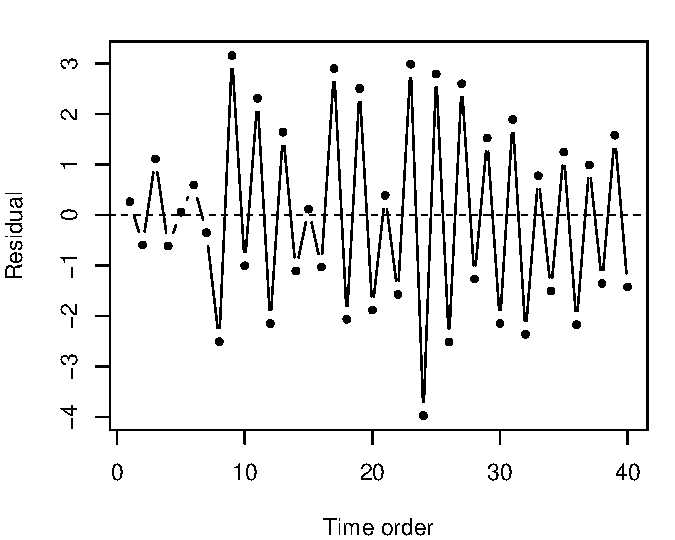
\includegraphics[width=0.75\linewidth]{figures/time-negative}}\mode<article>{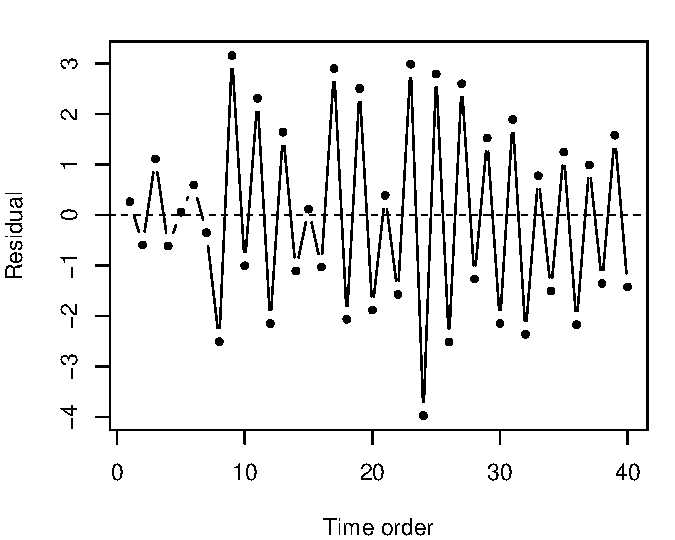
\includegraphics[width=0.8\linewidth]{figures/time-negative}}

        Negative autocorrelation: signs alternate.
    \end{columns}

    \svspace{0.75em}

    A trend over time suggests a missing time-dependent regressor.
\end{frame}


\subsection{Durbin--Watson Test}


\begin{frame}{First-Order Autoregressive Errors}
    \[
        \varepsilon_t=\phi\,\varepsilon_{t-1}+a_t, \qquad |\phi|<1, \qquad a_t \overset{iid}{\sim} N(0,\sigma_a^2)
    \]
    \begin{align*}
        \mathrm{E}[\varepsilon_t] &= 0 \\
        \mathrm{Var}(\varepsilon_t) &= \frac{\sigma_a^2}{1-\phi^2} \\
        \mathrm{Corr}(\varepsilon_t,\varepsilon_{t+j}) &= \phi^{\,j}
    \end{align*}
    $\phi>0$: neighboring errors are similar (positive autocorrelation). $\phi<0$: they tend to alternate in sign.
\end{frame}


\begin{frame}{Consequences of Autocorrelated Errors}
    \begin{itemize}
        \item The least-squares estimators are still unbiased, but no longer have minimum variance
        \item MSE typically underestimates $\sigma^2$
        \item The standard errors of the coefficients are underestimated
        \item Confidence intervals and $t$, $F$ tests are no longer valid
    \end{itemize}
\end{frame}


\begin{frame}{Durbin--Watson Statistic}
    \begin{align}
        d &= \frac{\sum_{t=2}^n (e_t-e_{t-1})^2}{\sum_{t=1}^n e_t^2} \label{eq:dw} \\
        &\approx 2(1-r_1), \qquad r_1=\frac{\sum_{t=2}^n e_te_{t-1}}{\sum_{t=1}^n e_t^2} \notag
    \end{align}
    \begin{itemize}
        \item $r_1$ is the lag-1 sample autocorrelation of the residuals
        \item $0\le d\le 4$
        \item $d\approx 2$: no autocorrelation; $d<2$: positive; $d>2$: negative
    \end{itemize}
\end{frame}


\begin{frame}{Why $d\approx 2(1-r_1)$?}
    Start from the numerator of \eqref{eq:dw}, $\sum_{t=2}^n (e_t-e_{t-1})^2$. Where does $2(1-r_1)$ come from?

    % Expand $(e_t-e_{t-1})^2=e_t^2+e_{t-1}^2-2e_te_{t-1}$. Sums of $e_t^2$ and $e_{t-1}^2$ over $t=2,\dots,n$ each differ from $\sum_{t=1}^n e_t^2$ by a single end term, so the numerator is approximately $2\sum e_t^2-2\sum e_te_{t-1}$. Dividing by $\sum e_t^2$ gives $2-2r_1$.
\end{frame}


\begin{frame}{Decision Rule}
    Test $H_0:\phi=0$ against $H_1:\phi>0$. The bounds $d_L$ and $d_U$ depend on $n$, the number of regressors $k$ and $\alpha$, and are tabulated.
    \begin{itemize}
        \item $d<d_L$: reject $H_0$, positive autocorrelation
        \item $d>d_U$: do not reject $H_0$
        \item $d_L\le d\le d_U$: inconclusive
    \end{itemize}
    For $H_1:\phi<0$ apply the same rule to $4-d$, with $d$ from \eqref{eq:dw}.
\end{frame}


\begin{frame}{Soft Drink Sales Data}
    \begin{columns}[T]
        \column{0.5\textwidth}
        \begin{itemize}
            \item $y$: annual sales in a sales region, $x$: annual advertising expenditure, $n=20$ years
            \item Fitted model: $\hat y=1608.5+20.091\,x$
            \item $d=1.08$
            \item $\alpha=0.05$, $n=20$, $k=1$: $d_L=1.20$, $d_U=1.41$
            \item $d<d_L$: reject $H_0$, evidence of positive autocorrelation
        \end{itemize}
        \column{0.47\textwidth}
        \centering
        \mode<presentation>{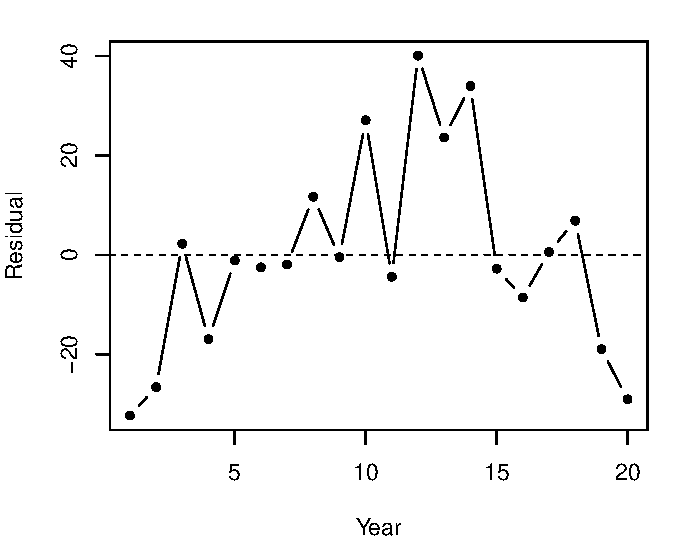
\includegraphics[width=\linewidth]{figures/softdrink-time}}\mode<article>{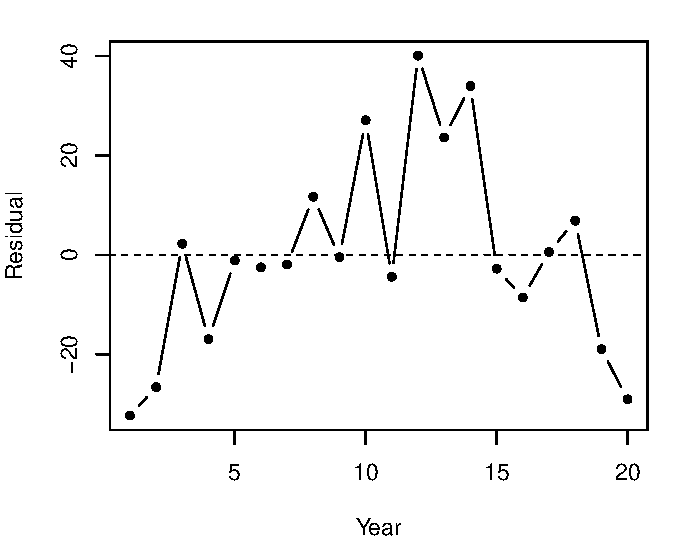
\includegraphics[width=0.7\linewidth]{figures/softdrink-time}}

        The plot alone is hard to judge by eye.
    \end{columns}
\end{frame}


\begin{frame}{If the Errors Are Autocorrelated}
    \begin{itemize}
        \item First look for a missing regressor, often a time-related one
        \item Otherwise estimate the model with an iterative procedure such as Cochrane--Orcutt (MPV, Chapter 14)
    \end{itemize}
\end{frame}


\section{Summary}


\begin{frame}{Diagnostics at a Glance}
    \mode<presentation>{\footnotesize}
    \begin{center}
        \begin{tabular}{lll}
            \toprule
            Tool & Checks & Typical remedy \\
            \midrule
            Normal plot, Shapiro--Wilk & Normal errors & Transform $y$ \\
            Plot vs $\hat y_i$, Breusch--Pagan, White & Constant variance & Transform $y$, WLS \\
            Plot vs $\hat y_i$ and vs $x_j$ & Mean function & Add terms, transform \\
            Plot vs time, Durbin--Watson & Uncorrelated errors & Add regressor \\
            $r_i$, $t_i$, $e_{(i)}$ & Unusual observations & Investigate \\
            \bottomrule
        \end{tabular}
    \end{center}
\end{frame}


\begin{frame}{Workflow and Key Messages}
    \begin{enumerate}
        \item Fit the model and compute studentized and R-student residuals
        \item Plot: normal probability plot, against $\hat y_i$, against regressors, against time order
        \item Use formal tests to back up what the plots suggest
        \item Apply a remedy, refit, and check again
    \end{enumerate}
    \begin{itemize}
        \item Residuals are not the errors: they have unequal variances and are correlated
        \item Plots first, tests second; tests depend heavily on $n$
        \item A single observation can drive a rejection
    \end{itemize}
\end{frame}
